

\section{Experiments}
\label{experiments}
For our experiments, our training data is given by $(x_i, f(x_i))$, where $x_i$ are randomly chosen from a standard Gaussian in $\R^d$ and $f$ is a randomly generated neural network with weights chosen from a standard Gaussian. We run gradient descent (Algorithm \ref{GD}) on the empirical loss, with stepsize around $\alpha = 10^{-5}$, for $T = 10^6$ iterations. The nonlinearity used at each node is sigmoid from -1 to 1, including the output node, unlike the assumptions in the theoretical analysis. A random guess for the network will result in a mean squared error of around 1. Our experiments (see Fig~\ref{expconverge}) show that for depth-2 neural networks, even with non-linear outputs, the training error diminishes quickly to under $0.002$. This seems to hold even when the width, the number of hidden nodes, is substantially increased (even up to 125 nodes), but depth is held constant; although as the number of nodes increases, the rate of decrease is slower. This substantiates our claim that depth-2 neural networks are learnable.

However, it seems that for depth greater than 2, the test error becomes significant  when width is high (see Fig~\ref{tablePlot}). Even for depth 3 networks, the increase in depth impedes the learnability of the neural network and the training error does not get close enough to 0. It seems that for neural networks with greater depth, positive convergence results in practice are elusive. We note that we are using training error as a measure of success, so it's possible that the true underlying parameters are not learned. 

\begin{figure}[!ht]
  \centering
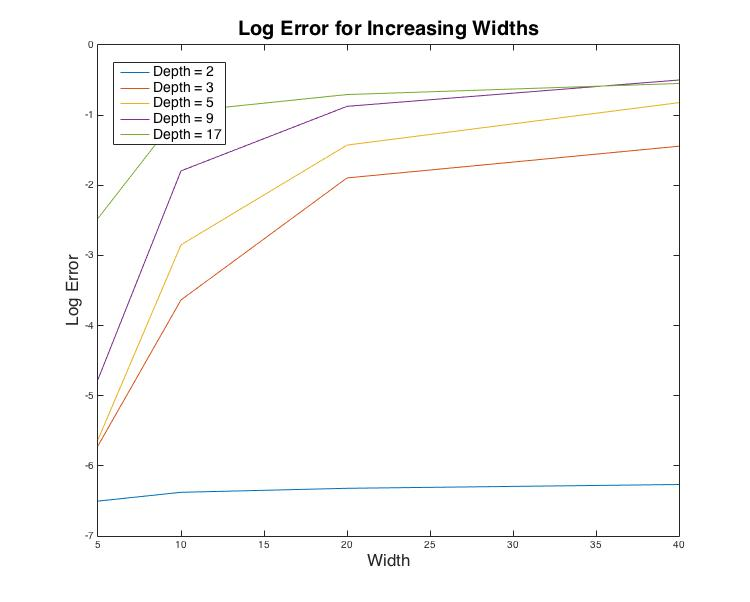
\includegraphics[width = 4.5in]{tablePlot.jpg}
\caption{Test Error of Varying-Depth Networks vs. Width}
\label{tablePlot}
\end{figure}

\begin{table}
\vskip 0.1in
\begin{center}
\begin{small}
\begin{sc}
\begin{tabular}{
  |p{\dimexpr.2\linewidth-2\tabcolsep-1.3333\arrayrulewidth}|% column 0
   |p{\dimexpr.2\linewidth-2\tabcolsep-1.3333\arrayrulewidth}% column 1
  |p{\dimexpr.2\linewidth-2\tabcolsep-1.3333\arrayrulewidth}% column 2
  |p{\dimexpr.2\linewidth-2\tabcolsep-1.3333\arrayrulewidth}% column 3
  |p{\dimexpr.2\linewidth-2\tabcolsep-1.3333\arrayrulewidth}% column 4
   |p{\dimexpr.2\linewidth-2\tabcolsep-1.3333\arrayrulewidth}% column 5
  }
   \hline 
           & Width 5   &  Width 10   & Width 20 & Width 40     \\ \hline 
    Depth 2 & 0.0015   & 0.0017      &   0.0018 & 0.0019 \\ \hline
    Depth 3 & 0.0033   & 0.0264        &   0.1503 & 0.2362 \\ \hline
    Depth 5 & 0.0036   & 0.0579        &   0.2400 & 0.4397 \\ \hline
    Depth 9 & 0.0085   & 0.1662        &   0.4171 & 0.6071 \\ \hline
    Depth 17 & 0.0845   & 0.3862        &   0.4934 & 0.5777 \\ \hline
\end{tabular}
\end{sc}
\end{small}
\end{center}
\caption{Test Error of Learning Neural Networks of Various Depth and Width}
\vskip -0.1in
\end{table}

% If our loss function were strongly convex, small training
% error would imply a small norm in the parameter space. 


% \Snote{Do we need the figure? Figures should be the same size. Make the fonts larger, they
%   are hard to read. The figure caption should read training error
%   rather than test error.}
%\begin{figure}[h!]
%  \centering
%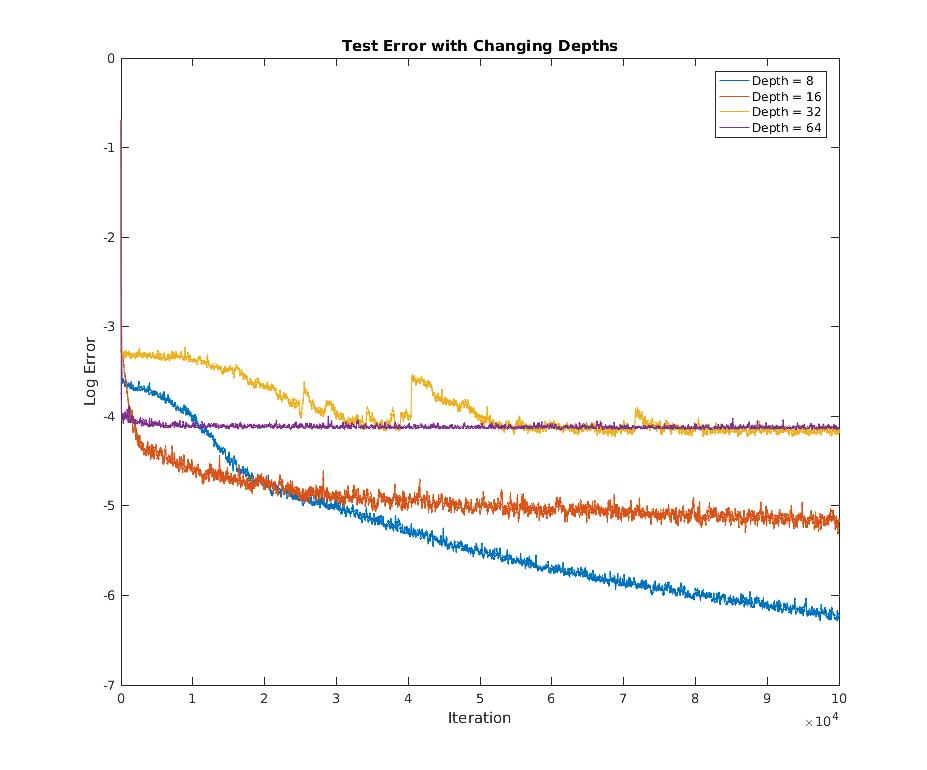
\includegraphics[width = 3.2in]{plotChangeDepth.jpg}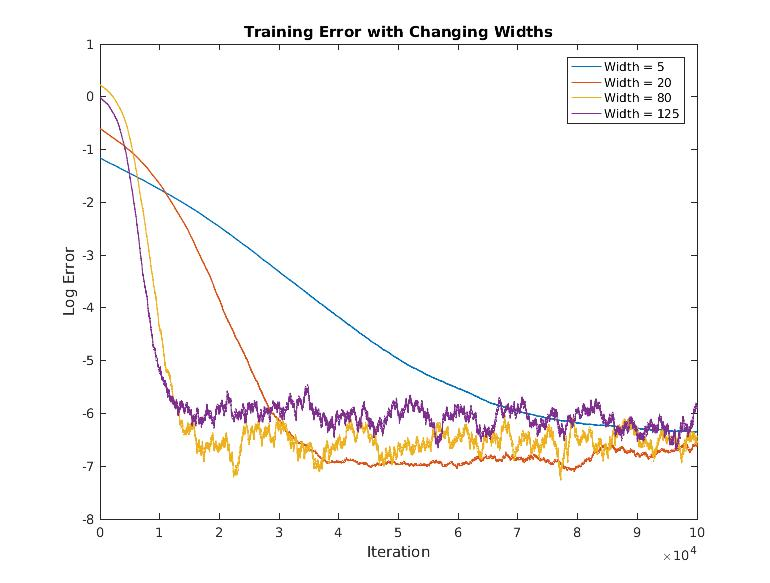
\includegraphics[width = 3.5in]{plotChangeWidth.jpg}
%\caption{Test Error of Varying-Depth Networks vs. Width} 
%%  \fbox{\rule[-.5cm]{0cm}{4cm} \rule[-.5cm]{4cm}{0cm}}
%\end{figure}


%%% Local Variables:
%%% mode: latex
%%% TeX-master: "icmlpaper2017.tex"
%%% End: